\section{Analysis}
\label{sec:ana}
\begin{figure}
    \centering
    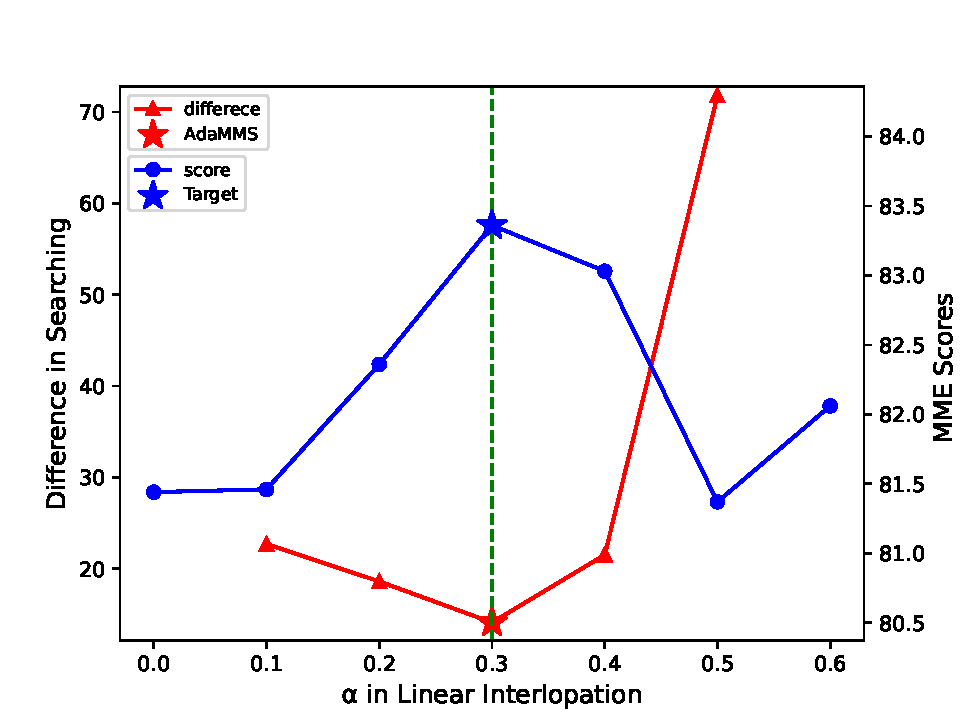
\includegraphics[width=0.4 \textwidth, bb=0 0 461 346]{figure/diff_acc_plot_new.pdf}
    \caption{Results on merging LLaVA-v1.5-7B into Qwen2-VL-7B. The $\alpha$ with the best perfo, bb=0 0 461 346rmance are the same as the $\alpha$ with the fewest response differences.}
    \label{fig:difference}
\end{figure}

%同构模型融合,以及searching方法的有效性。
\subsection{Different Factors for Calculating Generation Consistency}
We conducted analytical experiments on our generation consistency calculation methods, focusing on two key factors: the choice between using a 100-sample subset versus the complete dataset, and the selection of evaluation metrics. In the searching step of our method, we employed an exact match metric to calculate $\operatorname*{DiffCnt}$ in Algorithm~\ref{alg:composition}, which serves as our generation consistency indicator for model performance prediction. Given that exact match is a binary, rigorous evaluation metric, we explored an alternative, more flexible approach to measure generation consistency. Specifically, we computed the cosine similarity between sentence embeddings generated by all-MiniLM-L6-v2 \cite{sentence-bert}, which was used to calculate $\operatorname*{DiffCnt}$. The analysis results are presented in Table~\ref{tab:embedding}. Although embeddings theoretically offer more fine-grained semantic representations, our results demonstrate that the embedding-based metric performs comparably to the exact match metric. Furthermore, our experiments confirm that sampling 100 instances achieves results nearly equivalent to the complete dataset.


% In the searching step of \ours, we employed exact match metric to calculate $\operatorname*{DiffCnt}$ in Algorithm~\ref{alg:composition}, which is the the indicator of generation consistency that is used to predict the model performance.
% Since exact match is a binary, hard-judgment metric, we investigate an alternative, softer metric to capture generation consistency. Specifically, we compute the cosine similarity between sentence embeddings generated by all-MiniLM-L6-v2 \cite{sentence-bert}, which we use to calculate $\operatorname*{DiffCnt}$.
% % Given that the model often produces responses in sentence format, we incorporated embedding method to assess the consistency of responses, aiming to compare the effectiveness of these two evaluation approaches. 
% While embeddings theoretically offer a fine-grained semantic representation, the results depicted in Table \ref{tab:embedding} reveal that the embedding metric performs similarly with the exact match metric.
% % This disparity can be attributed to the fact that the consistency evaluated by the embedding metric does not correspond to alterations in the models' hidden states.
% % The initial assumption was that the responses from both models would identical, indicating similarity in their hidden states and loss, thereby illustrating a smoother model within the vicinity of that alpha value in the linear interpolation space.
% This indicates that our choice in the main experiments of the exact match metric is sufficient for demonstrating the generation consistency for performance estimation.


\subsection{Merging with Large Performance Gap}

As discussed in Section~\ref{sec:results}, all model merging methods experience performance drop after the merging on two benchmarks, OCRBench and TextVQA. It shows that merging a model with significant \textit{lower} performance into the base model will decrease the performance on the task. Conversely, in Table~\ref{tab:reverse}, the merging from Qwen2-VL-7B to LLaVA-OneVision-7B shows that merging a model with significant \textit{higher} performance into the base model will not necessarily improve the model performance. And in this case, \ours is the only model merging method that resists the performance drop after merging.
In general, we observed that original models with similar performance tends to benefit from model merging, while original models with large performance gap do not.

\begin{figure}
    \centering
    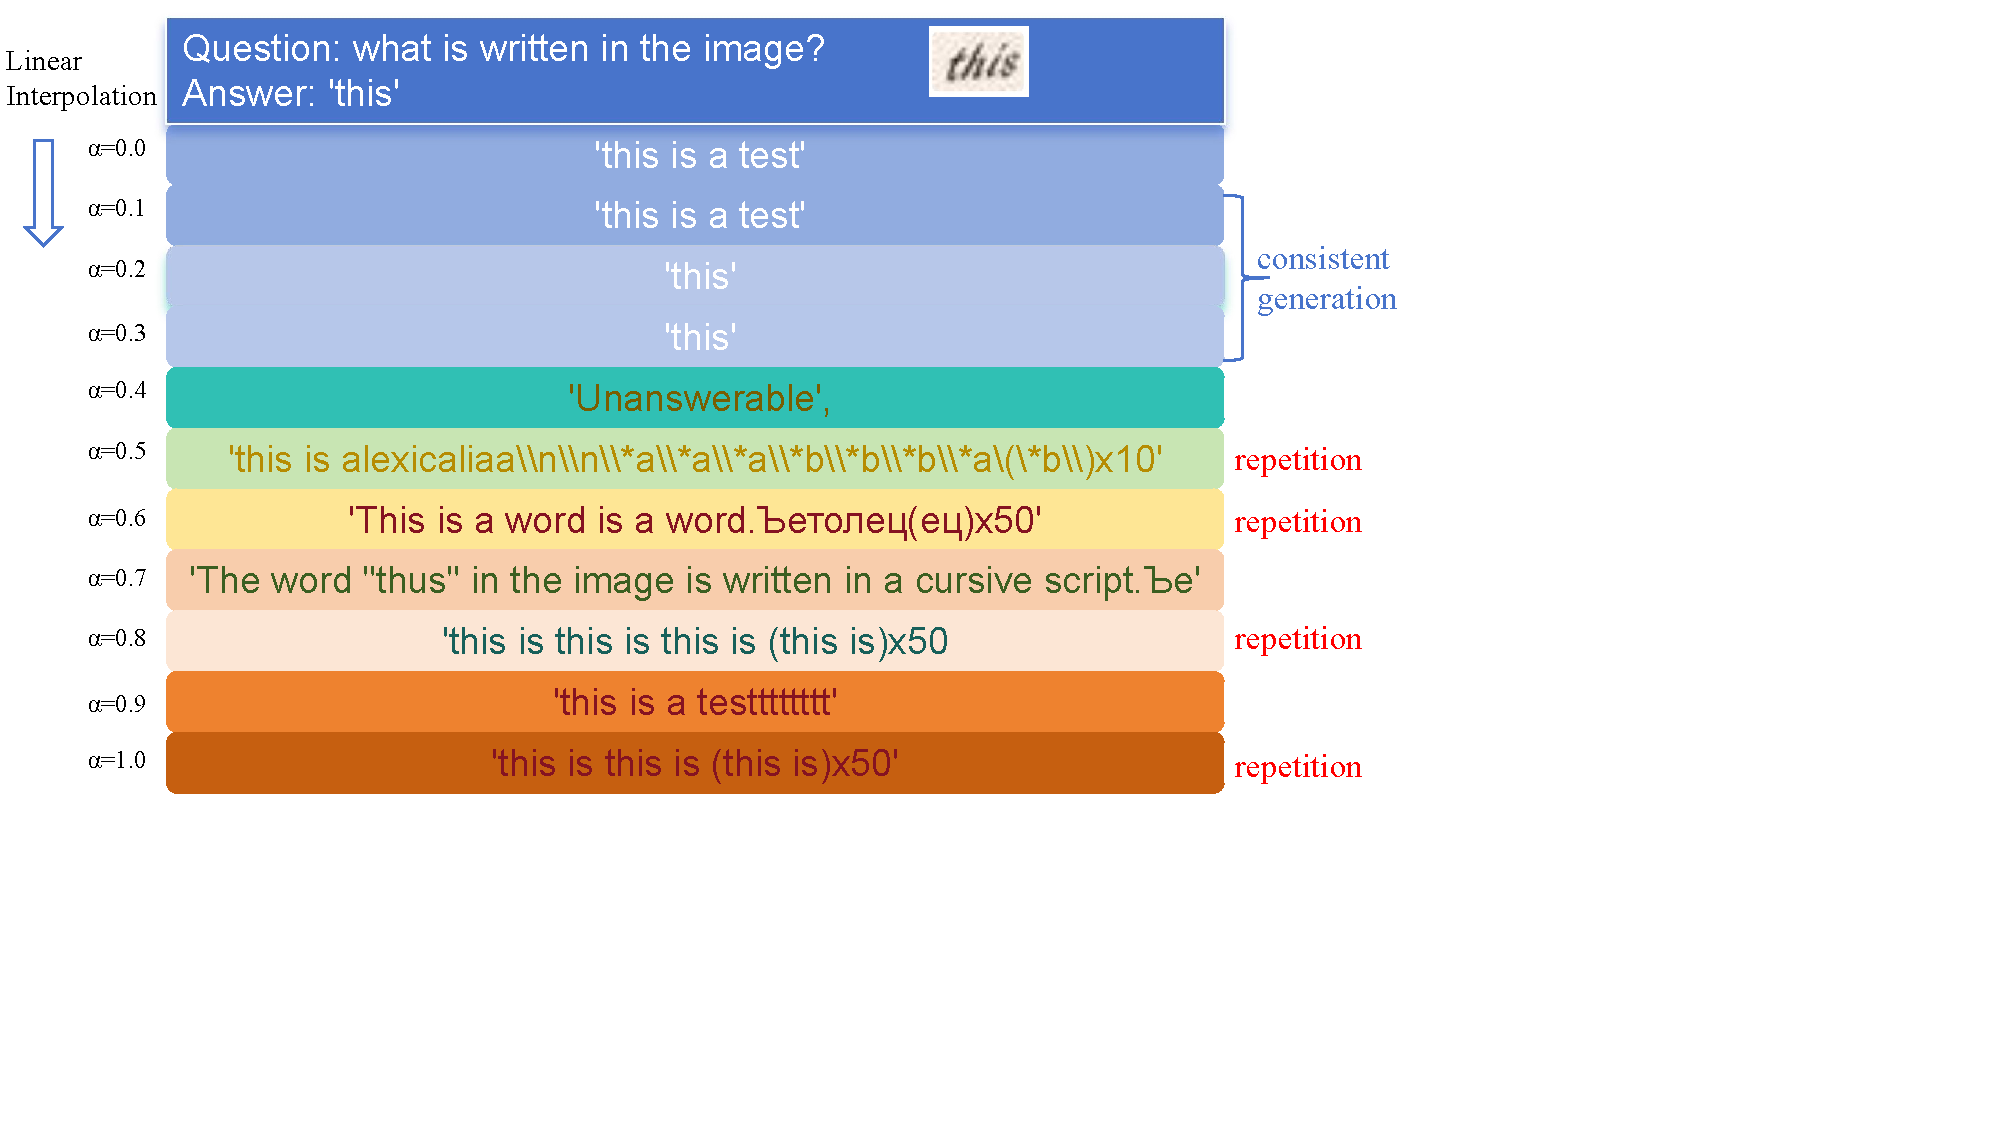
\includegraphics[width=\linewidth, bb=0 0 678 389]{figure/crop_diff-case.pdf}
    \caption{Model responses with the change of $\alpha$ in linear interpolation. Similar colors indicate similar responses.  }
    \label{fig:asymmetry}
\end{figure}

% The training data for different MLLMs varies, leading to performance differences across tasks. Model performance tends to be more stable when merging on tasks with smaller differences. Conversely, merging on tasks with large gap tends to unstable performance. Our mms-merging method exhibits strong stability, preventing models with poor performance from dragging down the overall results. As shown in Table \ref{tab:llava2qwen}  there is a 17\% gap between the two models for OCRBench \cite{ocrbench}. Only our mms-merging and MetaGPT \cite{metagpt} methods maintain the high performance of Qwen2\_VL \cite{Qwen2-VL-7B}.
%不同的MLLM训练数据不一样,这就导致了他们在任务上的表现有差异。在差异小的任务上进行融合时模型表现会比较稳定。而在差异大的任务进行融合则会表现动荡。 我们的方法具有很好的稳定性,可以避免表现差的模型拉低结果。可以看到表1中的OCRBENCH,两个模型相差17%,只有我们的mms-merging和metagpt保持住qwen2的好表现。
\subsection{Asymmetry in the Parameter Space of Heterogeneous Models} \label{sec:asymmetry_sec}
In Section~\ref{impl}, we discussed that merging with large $\alpha$ often results in collapsing language ability. To validate our choice of the subinterval $[0, 0.6]$ in determining candidates of $\alpha$, we demonstrate this phenomenon in Figure~\ref{fig:asymmetry}, which shows that the model generates consistently near the parameters of the base model with small $\alpha$, and collapses gradually with larger $\alpha$. We attribute the phenomenon to the asymmetry in the parameter space, as the two original models have unequal status that comes from the choice of base architecture.

\subsection{Selection of Granularity for \texorpdfstring{$\alpha$}{alpha}}
\label{sec:interval}
To validate our choice of the granularity in Section~\ref{impl}, we conducted additional experiments with various granularities of $\alpha$ candidates on n MME and OCRBench when merging LLaVA-OneVison-7B into Qwen2-VL-7B. As shown in Appendix~\ref{appendix:granularity}, the result shows that the difference of selected $\alpha$ and model performance do not change significantly with different granularities. This shows that our choice of granularity as 0.1 would result in comparable performance, with less computation cost.

% Generally speaking, there is a trade-off between the granularity of $\alpha$ and the results. The finer grained the alpha, the better the potential outcomes, but the higher the cost. In practice, we found that refining the granularity of $\alpha$  to 0.05 or 0.02 did not result in significant improvements. They are displayed in the Figure \ref{sec:interval}. Therefore selecting an interval of 0.1 for alpha in the main experiment was sufficient.





% \subsection{Homogeneous V.S. Heterogeneous Merging}
% % 我们的diff方法在同构模型中仍然有效。需要强调的是同构模型融合的所有结果增益都比较小,不如异构融合带来的增益。
% Both ShareGPT4V and LLaVA-1.5 include three integral components:(1)A vision encoder utilizing the CLIP-Large model.(2) A projector, two layer multi-layer perception (MLP),  to connect the vision and language modalities. (3) A LLM derived from LLaMA2.

% The merging method applied to these two homogeneous MLLMs is identical to that used on homogeneous LLMs. The results after merging remain stable, but the improvements are minimal. Therefore, we argue that the gains of merging heterogeneous MLLMs surpass homogeneous ones.
% 
\begin{table*}[!ht]
    \centering
    \resizebox{\textwidth}{!}{%
    \begin{tabular}{llllllllll}
    \toprule
     \textbf{Model} & $\mathrm{MMMU_{val}}$ &  $\mathrm{MME_{sum}}$ &  $\mathrm{SeedBench_{all}}$ & $\mathrm{OCRBench}$  &  $\mathrm{TextVQA_{val}}$  & $\mathrm{OKVQA}$ & $\mathrm{GQA}$  &  $\mathrm{VizWiz_{val}}$ & $\mathrm{SUM}$ \\ 
        \midrule
     0.0(Sharegpt) & 36.60  & 65.32  & 63.72  & 37.60  & 46.88  & 50.98  & 63.27  & 60.38  & 424.75  \\ 
        0.1 & 36.20  & 65.94  & 63.77  & 37.70  & 47.11  & 52.31  & 63.35  & 60.30  & 426.68  \\ 
        0.2 & 36.90  & 66.32  & 63.73  & 37.40  & 47.28  & 53.78  & 63.40  & 60.55  & 429.36  \\ 
        0.3 & 35.80  & 67.13  & 63.42  & 37.30  & 47.42  & 54.14  & 63.44  & 60.42  & 429.07  \\ 
        0.4 & 36.20  & 67.20  & 63.29  & 37.20  & 47.60  & 54.51  & 63.29  & 59.85  & 429.14  \\ 
        0.5 & 36.40  & 67.63  & 63.39  & 37.20  & 47.58  & 54.60  & 63.13  & 59.37  & 429.30  \\ 
        0.6 & 37.10  & 67.20  & 63.22  & 36.80  & 47.28  & 54.65  & 62.95  & 59.18  & 428.38  \\ 
        0.7 & 37.00  & 66.51  & 63.10  & 36.70  & 46.93  & 54.67  & 62.77  & 58.64  & 426.32  \\ 
        0.8 & 36.30  & 66.24  & 62.95  & 36.50  & 46.78  & 54.53  & 62.70  & 58.10  & 424.10  \\ 
        0.9 & 36.30  & 66.48  & 62.72  & 35.60  & 46.44  & 53.82  & 62.57  & 57.41  & 421.34  \\ 
        1.0(LLaVA) & 34.90  & 67.42  & 62.20  & 34.60  & 46.04  & 53.05  & 62.32  & 56.81  & 417.34  \\ 
        Task Arithmetic  & 36.10  & 69.61  & 63.40  & 37.00  & 50.65  & 53.37  & 63.13  & 59.29  & 432.55  \\ 
        Ties-Merging  & 35.90  & 69.57  & 61.73  & 35.70  & 50.36  & 54.44  & 63.17  & 54.89  & 425.76  \\ 
        DARE-Linear  & 36.30  & 69.40  & 63.36  & 37.40  & 50.70  & 53.71  & 63.06  & 59.55  & 433.48  \\ 
        DARE-Ties  & 32.80  & 58.59  & 56.49  & 32.60  & 44.11  & 50.20  & 57.23  & 43.78  & 375.80  \\ 
        MetaGPT & 36.30  & 70.58  & 63.44  & 37.10  & 50.93  & 53.57  & 63.23  & 59.72  & 434.87  \\ 
        diff3-sample0.1-EM & 36.30  & 66.48  & 63.77  & 37.30  & 47.60  & 54.14  & 63.13  & 60.55  & 429.27 \\ 
        \bottomrule
    \end{tabular}%
        }
    \caption{Results on various benchmark when merging LLaVA-v1.5-7B into ShareGPT-4V-7B.}
     \label{tab:llava2share}

\end{table*}



% \begin{figure}
%   \centering 
%  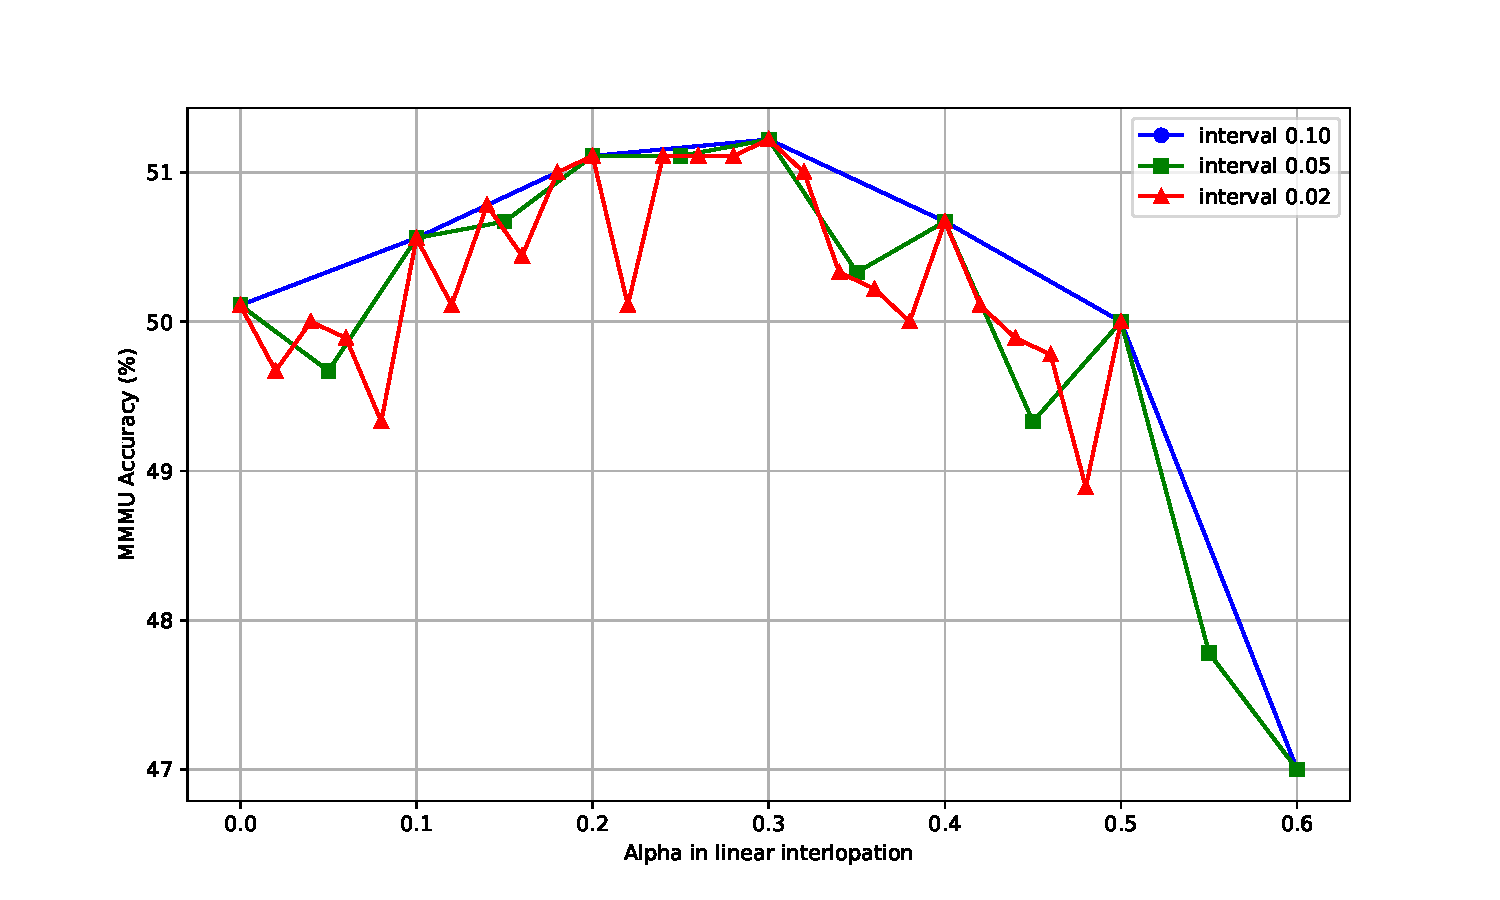
\includegraphics[width=0.4\textwidth]{figure/mmmu_mme_ocr.pdf}
%   \caption{Results with alpha intervals of 0.1, 0.05, and 0.02 in linear interpolation.}
%   \label{intervals}
% \end{figure}



 % 
\begin{table*}[!ht]
    \centering
    \resizebox{\textwidth}{!}{%
    \begin{tabular}{lclllllllllc}
        \toprule             

        Model & $\mathrm{Unsupervised}$ & $\mathrm{MMMU_{val}}$ &  $\mathrm{MME_{sum}}$ &  $\mathrm{SeedBench_{all}}$ & $\mathrm{OCRBench}$  &  $\mathrm{TextVQA_{val}}$  & $\mathrm{OKVQA}$ & $\mathrm{GQA}$  &  $\mathrm{VizWiz_{val}}$ & $\mathrm{SUM}$  & $\mathrm{Top2}$  \\ 
        \hline

\rowcolor{gray!20}
\multicolumn{12}{c}{\textbf{Original Models}} \\
\hline
 mPLUG-Owl2\footnotesize(base) & ~ & 34.90  & 62.80  & 59.41  & 34.10  & 55.13  & 60.98  & 56.11  & 32.07  & 395.50  \\ 
     CogVLM & ~  & 34.80  & 59.23  & 61.22  & \textit{56.50}  & \textit{77.57}  & 60.82  & \textit{59.43}  & \textit{37.09}  & \textit{446.66} \\ 
       
    
     \hline
       
\rowcolor{gray!20}
\multicolumn{12}{c}{\textbf{Baselines}} \\
\hline
Task Arithmetic &$\times$ & \underline{38.80\footnotesize(+3.95)} & \textbf{64.65\footnotesize(+3.63)} & \textbf{60.85\footnotesize(+0.53)} & \textbf{31.50\footnotesize(-13.80)} & \textbf{56.99\footnotesize(-9.36)} & 60.93\footnotesize(+0.03) & \underline{54.44\footnotesize(-3.33)} & \textbf{32.76\footnotesize(-1.82)} & \textbf{400.92\footnotesize(-20.16)} & 8 \\

        Ties-Merging &$\times$ & 27.9\footnotesize(-6.95) & 48.96\footnotesize(-12.06) & 52.32\footnotesize(-8.00) & 24.30\footnotesize(-21.00) & 42.10\footnotesize(-24.25) & 54.15\footnotesize(-6.75) & 43.02\footnotesize(-14.75) & 27.56\footnotesize(-7.02) & 320.31\footnotesize(-100.77) &0 \\ 
        
        DARE-Linear & $\times$ &37.60\footnotesize(+2.75) & 62.44\footnotesize(+1.42) & 59.81\footnotesize(-0.51) & 30.90\footnotesize(-14.40) & 56.41\footnotesize(-9.94) & \underline{61.07\footnotesize(+0.17)} & 54.11\footnotesize(-3.66) & 32.42\footnotesize(-2.16) & 394.76\footnotesize(-26.32) & 1\\ 
        
        DARE-Ties & $\times$ &32.00\footnotesize(-2.85) & 57.90\footnotesize(-3.12) & 57.62\footnotesize(-2.70) & 24.10\footnotesize(-21.20) & 43.84\footnotesize(-22.51) & 51.56\footnotesize(-9.34) & 52.04\footnotesize(-5.73) & 25.67\footnotesize(-8.91) & 344.73\footnotesize(-76.35) & 0\\
        
        MetaGPT & $\checkmark$&31.30\footnotesize(-3.55) & 56.81\footnotesize(-4.21) & 50.81\footnotesize(-9.51) & 29.30\footnotesize(-16.00) & 37.96\footnotesize(-28.39) & 43.02\footnotesize(-17.88) & 34.12\footnotesize(-23.65) & 15.84\footnotesize(-18.74) & 299.16\footnotesize(-121.92)  &0
          \\[0.5ex] 
               \hline       
\rowcolor{gray!20}
\multicolumn{12}{c}{\textbf{Our Method}} \\
\hline                    
       AdaMMS &$\checkmark$& \textbf{39.10\footnotesize(+4.25)} & \textbf{64.65\footnotesize(+3.63)} & \underline{60.16\footnotesize(-0.16)} & \underline{30.60\footnotesize(-14.70)} & \underline{55.88\footnotesize(-10.47)} & \textbf{62.11\footnotesize(+1.21)} & \textbf{55.61\footnotesize(-2.16)} & \underline{32.69\footnotesize(-1.89)} & \underline{400.80\footnotesize(-20.28)} & 9\\
        \bottomrule
    \end{tabular}%
        }
    \caption{Results on merging CogVLM-7B into mPLUG-Owl2-7B.}
    \label{tab:cog2mplug}
\end{table*}



% \input{floats/llava2mplug}